\section{Experiments}\label{sec:experiments}

The package \texttt{rareprob} (Python, numpy) implements the procedures above, with
the simplifications stated where they are described (a fixed atom size $a=12$ and fixed
(R7) constants in DFSB, a greedy elimination order, and the subset of modules run by the
meta-procedure, \cref{sec:modules}):
bit-parallel circuit evaluation, NNF conversion with small-cone
canonicalisation, the envelope compiler and estimator with boxes, DFSB and the
meta-procedure, context-width compilation, variable elimination, exponential tilting,
the Harris--Janson sandwich, certified telescoping, the tilted Glauber estimator, the
affine presolve and affine envelopes, Gaussian-elimination forcing, a
two-watched-literal DRUP checker, the PCIS verifier for envelope arguments with an
honest prover that calls a CDCL solver with proof logging, and the XPT verifier.
It simplifies some procedures: it fixes the atom size at $a=12$, uses greedy
elimination orders, replaces the pilot of the tilted Glauber estimator by a heuristic
one, and expands only threshold gates with nonnegative integer weights (others are
opaque); none of this affects soundness. Intervals are computed as in the
proofs (Hoeffding--KL intervals combined by union bounds, and the Bernstein and Maurer
bounds of \cref{sec:local}). Monte Carlo cost is not simulated for tiny $p$: we report
the number of samples its KL interval needs, at the same $(\eps,\delta)$, when the
empirical mean equals $p$ (this favours Monte Carlo). Scripts are in
\texttt{experiments/}, and each table and figure is generated from the raw output of
the script named in its caption.

\paragraph{Soundness (\cref{tab:coverage}).} We ran each procedure many times at
$\delta=0.1$ on random circuits and on families with exactly known $p$ (by
enumeration, inclusion--exclusion or dynamic programming), and counted intervals
that miss $p$. Adversarial arguments were included: a wrong envelope (a dropped
term) with the honest proof of the right envelope, a wrong envelope with a list of
random clauses as ``proof'', and an envelope disjoint from most of $C$'s mass with no
proof. Every miss rate is below $\delta$, as it must be; most are $0$, because the
union bounds and KL intervals are conservative.

\begin{table}[ht]
\centering\small
\begin{tabular}{lrrr}
\toprule
procedure & trials & misses & miss rate\\
\midrule
envelope (auto) on random circuits & 300 & 0 & 0.000\\
DFSB on random circuits & 150 & 2 & 0.013\\
KLM envelope on DNFs & 300 & 0 & 0.000\\
envelope with boxes on block products & 100 & 0 & 0.000\\
exponential tilting on thresholds & 200 & 0 & 0.000\\
Harris-Janson sandwich (deterministic) & 300 & 0 & 0.000\\
argument: honest envelope + DRUP proof & 150 & 0 & 0.000\\
argument: wrong envelope + stale proof & 150 & 0 & 0.000\\
argument: wrong envelope + bogus proof & 150 & 0 & 0.000\\
argument: disjoint envelope, no proof & 150 & 0 & 0.000\\
\bottomrule
\end{tabular}

\caption{Empirical miss rates at $\delta=0.1$ (\texttt{exp\_coverage.py}).}
\label{tab:coverage}
\end{table}

\paragraph{Cost versus rarity (\cref{fig:speedup}, \cref{tab:speedup}).}
Four families with exactly known $p$, at $\eps=0.1$, $\delta=0.05$:
\begin{itemize}
\item \emph{obfuscated DNF}: 16 random terms of width $w$ over 64 variables,
every literal routed through $(x\oplus r)\oplus r$ gadgets, terms built as trees,
the $\vee$ written as $\neg\wedge\neg$. Small-cone canonicalisation recovers the
literals and the envelope is the DNF itself ($K\approx1$);
\item \emph{triggers}: $R(x_{\rm body})\wedge[x_A=a]$ with the test written as
$\neg(x_i\oplus a_i)$ gates and $R$ a dense random circuit; forcing finds $x_A=a$;
\item \emph{products of blocks}: $\bigwedge_{j\le t}B_j$ with $B_j$ random
12-gate circuits on disjoint 6-variable blocks; every block is an atom, so DFSB
computes $p$ exactly by (T$'$) and (D), with no samples (\cref{cor:dfsb}(a)); blocks
above the atom size would be dense leaves, sampled with the $d^2$ accuracy split of
\cref{thm:dfsb};
\item \emph{thresholds of blocks}: $[\sum_jB_j\ge t]$ over $k$ random blocks,
by exponential tilting.
\end{itemize}
The cost of Monte Carlo grows like $2^{\sigma}$ in the surprise $\sigma=\log_2(1/p)$;
ours stays polynomial: flat for DNFs and triggers, zero samples for products of
atoms, and $O(\sqrt k)$ for thresholds.

\begin{figure}[ht]
\centering
\IfFileExists{figures/fig_speedup.pdf}{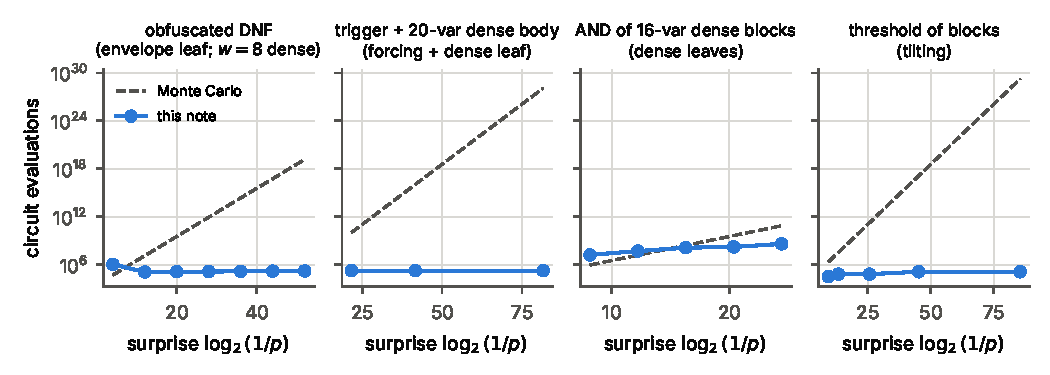
\includegraphics[width=\textwidth]{figures/fig_speedup.pdf}}{\fbox{figure pending}}
\caption{Circuit evaluations to reach an interval of ratio $\le1.1$ ($\eps=0.1$,
$\delta=0.05$) against the surprise $\log_2(1/p)$, compared with Monte Carlo's
requirement (\texttt{exp\_speedup.py}).}
\label{fig:speedup}
\end{figure}

\begin{table}[ht]
\centering\scriptsize
\begin{tabular}{llrrrrr}
\toprule
family & param & $p$ & interval ratio & cost & Monte Carlo & speed-up\\
\midrule
dnf-obfuscated & 8 & $6.08\cdot10^{-2}$ & 1.032 & $1.02\cdot10^{3}$ & $5.02\cdot10^{4}$ & $49.1$\\
dnf-obfuscated & 16 & $2.44\cdot10^{-4}$ & 1.073 & $6.55\cdot10^{4}$ & $1.33\cdot10^{7}$ & $2.03\cdot10^{2}$\\
dnf-obfuscated & 24 & $9.54\cdot10^{-7}$ & 1.083 & $1.00\cdot10^{6}$ & $3.41\cdot10^{9}$ & $3.41\cdot10^{3}$\\
dnf-obfuscated & 32 & $3.73\cdot10^{-9}$ & 1.808 & $1.00\cdot10^{6}$ & $8.73\cdot10^{11}$ & $8.73\cdot10^{5}$\\
dnf-obfuscated & 40 & $1.46\cdot10^{-11}$ & 270695.667 & $1.00\cdot10^{6}$ & $2.23\cdot10^{14}$ & $2.23\cdot10^{8}$\\
dnf-obfuscated & 48 & $5.68\cdot10^{-14}$ & inf & $1.00\cdot10^{6}$ & $5.72\cdot10^{16}$ & $5.72\cdot10^{10}$\\
trigger & 10 & $3.05\cdot10^{-4}$ & 1.087 & $1.02\cdot10^{3}$ & $1.06\cdot10^{7}$ & $1.04\cdot10^{4}$\\
trigger & 20 & $2.38\cdot10^{-7}$ & 1.004 & $1.02\cdot10^{3}$ & $1.36\cdot10^{10}$ & $1.33\cdot10^{7}$\\
trigger & 30 & $4.66\cdot10^{-10}$ & 1.091 & $4.10\cdot10^{3}$ & $6.98\cdot10^{12}$ & $1.70\cdot10^{9}$\\
trigger & 40 & $3.41\cdot10^{-13}$ & 1.087 & $2.05\cdot10^{3}$ & $9.53\cdot10^{15}$ & $4.65\cdot10^{12}$\\
trigger & 60 & $4.00\cdot10^{-19}$ & 1.066 & $1.45\cdot10^{5}$ & $8.13\cdot10^{21}$ & $5.61\cdot10^{16}$\\
trigger & 80 & $7.24\cdot10^{-25}$ & 1.029 & $1.92\cdot10^{4}$ & $4.49\cdot10^{27}$ & $2.34\cdot10^{23}$\\
blocks & 4 & $1.27\cdot10^{-2}$ & 1.082 & $8.19\cdot10^{3}$ & $2.53\cdot10^{5}$ & $30.9$\\
blocks & 8 & $1.85\cdot10^{-3}$ & 1.029 & $2.11\cdot10^{6}$ & $1.75\cdot10^{6}$ & $0.829$\\
blocks & 16 & $1.33\cdot10^{-5}$ & 1.066 & $5.88\cdot10^{6}$ & $2.45\cdot10^{8}$ & $41.7$\\
blocks & 24 & $3.86\cdot10^{-9}$ & 1.115 & $1.38\cdot10^{7}$ & $8.43\cdot10^{11}$ & $6.12\cdot10^{4}$\\
blocks & 32 & $3.62\cdot10^{-11}$ & 1.361 & $2.44\cdot10^{7}$ & $8.98\cdot10^{13}$ & $3.69\cdot10^{6}$\\
threshold & 50 & $5.59\cdot10^{-3}$ & 1.083 & $3.28\cdot10^{4}$ & $5.78\cdot10^{5}$ & $17.6$\\
threshold & 100 & $4.10\cdot10^{-5}$ & 1.087 & $3.28\cdot10^{4}$ & $7.92\cdot10^{7}$ & $2.42\cdot10^{3}$\\
threshold & 200 & $7.74\cdot10^{-8}$ & 1.089 & $6.55\cdot10^{4}$ & $4.20\cdot10^{10}$ & $6.41\cdot10^{5}$\\
threshold & 400 & $2.51\cdot10^{-15}$ & 1.079 & $1.31\cdot10^{5}$ & $1.29\cdot10^{18}$ & $9.87\cdot10^{12}$\\
threshold & 800 & $7.79\cdot10^{-27}$ & 1.096 & $3.28\cdot10^{4}$ & $4.17\cdot10^{29}$ & $1.27\cdot10^{25}$\\
\bottomrule
\end{tabular}

\caption{The runs of \cref{fig:speedup}. ``Cost'' counts all circuit evaluations,
including pilots and box estimation.}
\label{tab:speedup}
\end{table}

\paragraph{Context width (\cref{tab:ctx}).} ORs of $t$ CNFs with clauses on
sliding windows of width $w$, each CNF along its own random variable order, built as
left-deep $\wedge$-chains in window order (the bracketing of \cref{lem:pathcw}, kept by
the unflattened NNF). The compiler of \cref{thm:cw} finds context width $w$, the bound
of \cref{ex:or-cnf}, and produces an equivalent DNNF; the envelope estimator on it needs
only the minimum batch of $1{,}024$ samples, because the top $\vee$'s children are rare and almost
disjoint ($K\approx1$). Instances with $n\le24$ agree with enumeration.

\begin{table}[ht]
\centering\scriptsize
\IfFileExists{tables/ctx.tex}{\begin{tabular}{rrrrrrrrr}
\toprule
$n$ & $t$ & $w$ & cw & $|C|$ & DNNF size & interval for $p$ & samples & time (s)\\
\midrule
20 & 4 & 3 & 3 & 249 & 640 & [$0.39$, $0.416$] ($p=$0.393$$) & 1024 & 0.1\\
24 & 4 & 3 & 3 & 304 & 627 & [$0.209$, $0.221$] ($p=$0.215$$) & 1024 & 0.1\\
100 & 4 & 3 & 3 & 1375 & 2350 & [$9.50\cdot10^{-6}$, $9.54\cdot10^{-6}$] & 1024 & 0.6\\
200 & 4 & 3 & 3 & 2757 & 4575 & [$1.57\cdot10^{-11}$, $1.58\cdot10^{-11}$] & 1024 & 0.8\\
400 & 4 & 3 & 3 & 5633 & 8927 & [$2.91\cdot10^{-23}$, $2.92\cdot10^{-23}$] & 1024 & 2.1\\
800 & 8 & 3 & 3 & 22300 & 33927 & [$3.93\cdot10^{-46}$, $3.95\cdot10^{-46}$] & 1024 & 10.8\\
400 & 4 & 5 & 5 & 7115 & 15137 & [$1.46\cdot10^{-5}$, $1.46\cdot10^{-5}$] & 1024 & 6.0\\
\bottomrule
\end{tabular}
}{(table pending)}
\caption{Context-width compilation of ORs of window-CNFs (\texttt{exp\_ctx.py}).}
\label{tab:ctx}
\end{table}

\paragraph{Certified independence (\cref{tab:janson}).} Unate random $k$-CNFs with
up to $2\cdot10^5$ clauses: the Harris--Janson interval is deterministic, takes
seconds to a few minutes in Python, and on $200$ small instances it contained the exact
$p$ every time. At $n=2\cdot10^6$, $p\in[6.18,7.35]\cdot10^{-22}$; Monte Carlo would need
about $10^{24}$ evaluations for the same ratio. The second-order sandwich of
\cref{app:second-order} was checked against enumeration on 382 random instances with
no violations.

\begin{table}[ht]
\centering\scriptsize
\IfFileExists{tables/janson.tex}{\begin{tabular}{rrrrrr}
\toprule
$n$ & clauses & width & certified interval & ratio & time (s)\\
\midrule
10000 & 2000 & 10 & [$0.141$, $0.148$] & 1.039 & 0.8\\
100000 & 20000 & 12 & [$7.57\cdot10^{-3}$, $7.84\cdot10^{-3}$] & 1.035 & 11.0\\
200000 & 60000 & 12 & [$4.33\cdot10^{-7}$, $5.07\cdot10^{-7}$] & 1.167 & 50.3\\
1000000 & 200000 & 14 & [$4.99\cdot10^{-6}$, $5.15\cdot10^{-6}$] & 1.030 & 194.2\\
2000000 & 200000 & 12 & [$6.18\cdot10^{-22}$, $7.35\cdot10^{-22}$] & 1.187 & 71.0\\
\bottomrule
\end{tabular}
}{(table pending)}
\caption{Harris--Janson sandwich for random unate CNFs (\texttt{exp\_janson.py}).}
\label{tab:janson}
\end{table}

\paragraph{Certified telescoping (\cref{tab:cftp}).} Hard-core ladders: $x\sim
\mathrm{Bern}(0.3)^{n}$ and $C$ = ``$x$ is an independent set of the $2\times L$
ladder''. Janson's $\Delta$ is extensive, so the sandwich is useless; bounding-chain
CFTP gives exact samples, the truncation certificates contribute a bias factor below
$e^{0.02}$, and the certified intervals contain the exact $p$ (from variable
elimination).
In pure Python the constants are poor (each CFTP run costs thousands of updates), so
for these moderate $p$ Monte Carlo is still cheaper; the point is that the cost grows
polynomially in $L$ while $1/p$ grows exponentially, and that the method is sound
without any mixing-time proof.

\begin{table}[ht]
\centering\scriptsize
\IfFileExists{tables/cftp.tex}{\begin{tabular}{rrrlll}
\toprule
$L$ & $n$ & $p$ (exact) & Harris--Janson window & certified telescoping & CFTP runs\\
\midrule
20 & 40 & $2.31\cdot10^{-2}$ & [$4.21\cdot10^{-3}$, $0.107$] & [$2.07\cdot10^{-2}$, $2.69\cdot10^{-2}$] & $2.34\cdot10^{5}$\\
40 & 80 & $4.90\cdot10^{-4}$ & [$1.46\cdot10^{-5}$, $1.18\cdot10^{-2}$] & [$4.15\cdot10^{-4}$, $6.06\cdot10^{-4}$] & $4.42\cdot10^{5}$\\
60 & 120 & $1.04\cdot10^{-5}$ & [$5.12\cdot10^{-8}$, $1.31\cdot10^{-3}$] & [$8.36\cdot10^{-6}$, $1.35\cdot10^{-5}$] & $6.76\cdot10^{5}$\\
\bottomrule
\end{tabular}
}{(table pending)}
\caption{Certified telescoping on hard-core ladders (\texttt{exp\_cftp.py}).}
\label{tab:cftp}
\end{table}

\paragraph{Local thresholds (\cref{tab:local}).} \Cref{sec:local} reports the tilted
Glauber estimator on chain and random-cubic-graph local threshold circuits with random
local tables ($p$ down to $10^{-23.7}$ with certified Glauber samplers, and
$10^{-169.8}$ with coupling from the past beyond the Dobrushin regime), checked against
exact transfer-matrix values for chains and $10^7$ Monte Carlo samples for a small
cubic instance (\texttt{exp\_local.py}).

\paragraph{Affine structure (\cref{tab:affine}).} \Cref{sec:affine} reports the
presolve, affine envelopes, XPT arguments and DFSB on parity-check families under
uniform and biased product distributions, with exact values computed without the
module under test (\texttt{exp\_affine.py}).

\paragraph{What the prover adds (\cref{tab:arguments}, \cref{fig:proofs}).}
Hidden triggers $R\wedge T(x_S)$ whose test accepts only $x_S=a$:
\emph{linear-hash} tests $[Mx_S=Ma]$ with a dense $(k+4)\times k$ matrix over
$\F_2$, and \emph{SPN} tests $[\mathrm{SPN}(x_S)=\mathrm{SPN}(a)]$ with random
bijective 4-bit S-boxes and dense invertible linear layers. Without a prover,
Gaussian-elimination forcing recognises linear hashes. SPN tests are reached only
through small-cone canonicalisation: a test on at most $a=12$ variables is an atom
whose OBDD exposes $x_S=a$ to forcing, and DFSB reduces larger tests to atoms by
branching, with about $2^{|S|-a}$ leaves. With a prover, the argument is the subcube
$x_S=a$ plus a DRUP proof (from Glucose) that $C\Rightarrow(x_S=a)$; the verifier
checks it with its own RUP checker and samples only $R$. The DRUP proofs found by the
solver grow exponentially with $k$ even for linear hashes (CDCL solvers do not perform
Gaussian elimination); this is evidence, not a resolution lower bound, that the class
of \cref{thm:certenv} depends on the proof system.

\begin{table}[ht]
\centering\scriptsize
\IfFileExists{tables/arguments.tex}{\begin{tabular}{lrrrrrrr}
\toprule
family & $k$ & $|C|$ & $p$ & Part 1 ratio & proof steps & check (s) & Part 2 ratio\\
\midrule
linear hash & 12 & 78 & $1.53\cdot10^{-4}$ & 1 & 329 & 0.0 & 1.088\\
linear hash & 16 & 86 & $3.81\cdot10^{-6}$ & 1 & 1269 & 0.2 & 1.079\\
linear hash & 20 & 82 & $5.96\cdot10^{-7}$ & 1 & 5717 & 2.1 & 1.093\\
linear hash & 24 & 96 & $2.98\cdot10^{-8}$ & 1 & 32910 & 81.4 & 1.085\\
SPN, 2 rounds & 8 & 246 & $3.85\cdot10^{-3}$ & 1 & 278 & 0.0 & 1.027\\
SPN, 2 rounds & 12 & 334 & $1.37\cdot10^{-4}$ & 1 & 697 & 0.2 & 1.074\\
SPN, 3 rounds & 16 & 609 & $6.68\cdot10^{-6}$ & 1 & \multicolumn{3}{l}{no proof within 1200 s}\\
SPN, 3 rounds & 20 & 756 & $9.54\cdot10^{-7}$ & none in 900 s & 25944 & 39.5 & 1.004\\
\bottomrule
\end{tabular}
}{(table pending)}
\caption{Hidden triggers with and without a prover (\texttt{exp\_arguments.py}).
Part 1 ratio is that of the DFSB interval ($\infty$: lower end $0$); Part 2 ratio
is that of the verifier's interval after checking the proof.}
\label{tab:arguments}
\end{table}

\begin{figure}[ht]
\centering
\begin{minipage}{0.48\textwidth}\centering
\IfFileExists{figures/fig_proofs.pdf}{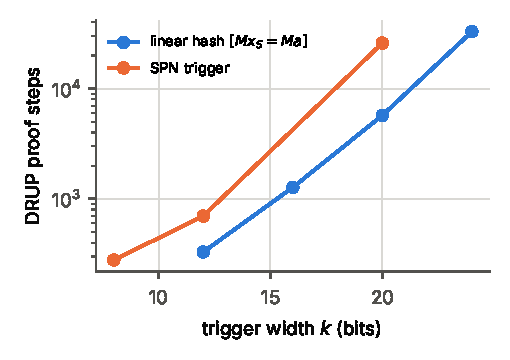
\includegraphics[width=\textwidth]{figures/fig_proofs.pdf}}{\fbox{figure pending}}
\caption{DRUP proof size for hidden triggers.}\label{fig:proofs}
\end{minipage}\hfill
\begin{minipage}{0.48\textwidth}\centering
\IfFileExists{figures/fig_surprise.pdf}{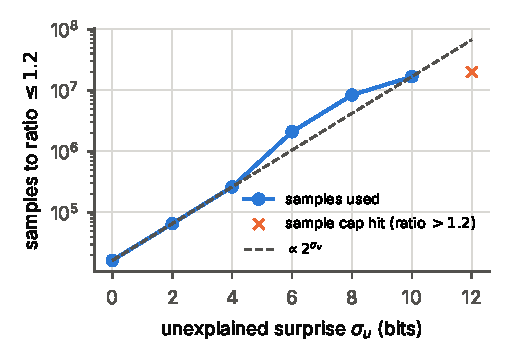
\includegraphics[width=\textwidth]{figures/fig_surprise.pdf}}{\fbox{figure pending}}
\caption{Surprise accounting: samples needed when an argument reveals all but
$\sigma_u$ bits of a 40-bit trigger.}\label{fig:surprise}
\end{minipage}
\end{figure}

\paragraph{Surprise accounting (\cref{fig:surprise}).} For a 40-bit trigger, an
argument that reveals $40-\sigma_u$ of the bits (a subcube envelope on those bits)
leaves $\sigma_u$ bits to sampling; the number of samples grows as $2^{\sigma_u}$, as
\cref{thm:surprise} says it must.
